\documentclass[conference]{IEEEtran}
\usepackage{graphicx}
\usepackage{booktabs}
\usepackage{amsmath}
\usepackage{amssymb}
\usepackage{url}
\usepackage[hidelinks]{hyperref}

\begin{document}
\title{From Diagnosis to Cure:\\
Decomposing the Tile-SPMD Abstraction Regret\\
on Irregular Automata}
\author{\IEEEauthorblockN{Anonymous}}
\maketitle

\begin{abstract}
Tile-based GPU DSLs (Triton) trail hand-written CUDA by ${\sim}10\times$ on irregular
finite-automata workloads. Prior work attributed this ``abstraction regret'' to the execution
\emph{paradigm} (tile/SPMD vs.\ thread-SIMT) rather than abstraction height. We turn that diagnosis
into an anatomy and a cure: we decompose the regret into three independently measured components and
identify, to the instruction level, the single missing primitive. On a work-efficient NFA worklist
the $10\times$ anchor decomposes as \textbf{(A)} a launch-configuration artifact (${\sim}3.4\times$,
default \texttt{num\_warps}), \textbf{(B)} a lane-packing-recoverable component (warp-redundant scalar
execution), and \textbf{(C)} an irreducible ${\sim}2\times$ residual. Component C is \emph{not}
instruction count, occupancy, or memory bandwidth: at matched occupancy and \emph{fewer}
warp-instructions than CUDA, and sitting below both the issue and bandwidth roofline ceilings, a
per-lane Triton worklist still spends $15.3\times$ more cycles in the dependent-load stall and issues
at $9.9\%$ vs.\ $41\%$ of peak---it is latency-bound. The root cause is abstraction-denied
intra-warp memory-level parallelism: a CUDA warp's lanes issue independent in-flight loads that
overlap, whereas a lock-step tile serializes the dependent next-state load. We show the residual is
\emph{regime-dependent}: for the memory-bound DFA it closes (lane-packed Triton matches CUDA,
$1.05\times$, once the table spills to DRAM). We specify the missing IR primitive---a
\texttt{scalar\_program} region that lowers each lane to an independent instruction stream---bound its
payoff, and give the thread-model existence proof. Every kernel is correctness-gated against a CPU
oracle; every number traces to a versioned CSV.
\end{abstract}

\section{Introduction and Contributions}
A companion study~\cite{paper1} shows that on irregular automata the Triton$\rightarrow$CUDA gap
follows the execution paradigm, not the abstraction height. It leaves open \emph{why}, mechanistically,
and \emph{what} would close it. This paper answers both. Our contributions:
\begin{enumerate}
\item A \textbf{falsifiable decomposition} of the tile-SPMD automata regret into artifact, recoverable,
and irreducible, each measured and Nsight-attributed (Sec.~\ref{sec:decomp}, Fig.~\ref{fig:decomp}).
\item Identification of the irreducible residual as \textbf{abstraction-denied intra-warp latency
hiding}---not redundancy, occupancy, instruction count, or bandwidth---\emph{measured}: fewer
warp-instructions than CUDA, same occupancy, below both roofline ceilings, yet $15.3\times$ the
dependent-load stall and $9.9\%$ vs.\ $41\%$ issue activity (Sec.~\ref{sec:resid}).
\item A demonstration that the residual is \textbf{regime-dependent} (latency-bound NFA vs.\
memory-bound DFA), unifying both faces through one latency mechanism (Sec.~\ref{sec:regime}).
\item A \textbf{launch-configuration finding} (default \texttt{num\_warps=4} inflates the worklist
regret ${\sim}3.4\times$), a methodological caution for DSL benchmarking (Sec.~\ref{sec:artifact}).
\item The \textbf{missing-primitive design} + a bound on its payoff + the thread-model existence proof,
distinguished from Gluon's per-thread \emph{layout} (Sec.~\ref{sec:cure}).
\end{enumerate}

\section{Background and Method}
NFA simulation (a work-efficient worklist iterating the active set via \texttt{ffs} over a bitmask) is
control-flow/latency-bound; DFA simulation (one dependent table gather \texttt{trans[cur*256+sym]} per
symbol) is memory-bound. CUDA and NVIDIA Warp~\cite{warp2022} are thread-SIMT (one thread per string);
Triton~\cite{triton2019} is tile/SPMD (a program operates on tiles). Correctness gates speed: every
kernel/config is validated bit-for-bit against a CPU oracle before any throughput is reported. We
report medians over warmup${+}9$ reps at a GPU-saturating batch~\cite{hoefler2015}, sweep batch (the
lane-packing benefit is occupancy-gated), and confirm the mechanism behind each claim with Nsight
Compute. Negative and partial results, and two corrected intermediate hypotheses, are reported.
Hardware: RTX 4070 (sm\_89), Triton 3.5.1, CUDA 13.3.

\section{The Decomposition (NFA worklist)}\label{sec:decomp}

\subsection{The anchor}
A work-efficient register-resident worklist ($\le 64$ states, batch 4096, 12 configs): Triton
$22$\,Gbps vs.\ CUDA $227$\,Gbps $=$ \textbf{$10.1\times$ median} ($9.4$--$12.3\times$).

\subsection{Component A: launch-configuration artifact}\label{sec:artifact}
The Triton worklist defaults to \texttt{num\_warps=4}: four warps per program redundantly process the
\emph{same} string. Sweeping \texttt{num\_warps}$\in\{1,2,4,8\}$: \texttt{nw=1} vs.\ \texttt{nw=4} $=$
$2.77\times$@4096 $\rightarrow 3.44\times$@16384 $\rightarrow 3.69\times$@65536 (each doubling
${\sim}$halves throughput). This inflates prior worklist regret numbers and must be disclosed.

\subsection{Component B: warp redundancy, recoverable by lane-packing}
The scalar Triton program executes warp-uniformly: \texttt{thread\_inst\_per\_inst} $=32.00$ (Triton)
vs.\ $30.34$ (CUDA), the same number with opposite meaning---CUDA's 32 lanes run 32 \emph{different}
strings, Triton's run the \emph{same} one---yielding ${\sim}90\times$ more warp-instructions. Lane-packing
(32 strings into the 32 lanes, exploiting the shared CSR so inner-loop bounds stay scalar) removes it.
On the dense scan, pure lane-packing recovers $3.2\times \rightarrow 9.8\times \rightarrow 19.4\times$
(batch 4096/16384/65536) toward the ideal $32\times$; it is \textbf{occupancy-gated}
(Fig.~\ref{fig:occ}). \emph{Correction:} we first framed the $90\times$ warp-redundancy as the
bottleneck; Nsight shows it is removed ${\sim}26\times$ yet throughput moves only $3.8\times$---it was
largely hidden by occupancy.

\subsection{Component C: the irreducible residual}\label{sec:resid}
A per-lane Triton worklist (each lane its own \texttt{ffs} + per-lane CSR gather, no cross-lane reduce,
no active-set union) beats the union variant $1.27\times$ but is still $0.51\times$ of CUDA
($\approx 2\times$ slower). Nsight is decisive (Fig.~\ref{fig:mech}): it has \emph{fewer}
warp-instructions than CUDA ($4.66$M vs.\ $5.07$M) and the same occupancy ($22.5\%$), yet is $3.3\times$
slower because issue activity is $9.9\%$. Raising occupancy does not help---a \texttt{BLOCK} sweep
$\{32,64,128,256\}$ only \emph{worsens} it ($0.49\times \rightarrow 0.31\times$): bigger lock-step
tiles add divergence. \textbf{Direct measurement} confirms the mechanism: at matched occupancy the
per-lane Triton kernel spends $15.3\times$ more cycles in the \texttt{long\_scoreboard} stall (waiting
on a dependent memory load) than CUDA, and the issue-rate ratio ($4.1\times$) tracks the throughput
ratio ($3.5\times$), consistent with Little's law~\cite{volkov2016latency,hongkim2009}. The
instruction roofline (Fig.~\ref{fig:roof})~\cite{instroofline2022} settles ``did you write a worse
kernel?'': both kernels sit far below the issue \emph{and} bandwidth ceilings ($8.3\%/27\%$ vs.\
$32\%/3.4\%$ of peak), and Triton issues fewer warp-instructions yet runs $3.5\times$ slower---it is
structurally latency-bound. \emph{Honest refinement:} the per-lane kernel does not issue \emph{fewer}
memory requests---it issues $26$--$84\times$ \emph{more} (masked inactive-lane gathers)---so the tile
model pays twice: excess masked traffic \emph{and} no dependent-load hiding. Root cause: a CUDA warp's
lanes are independent in-flight-load generators (memory-level parallelism); a lock-step tile serializes
the dependent next-state load, so latency hides only across warps (occupancy-bound). This is distinct
from branch/memory divergence~\cite{fung2007}: the lanes can be perfectly coalesced and still stall on
a dependent load. We distinguish it from the \emph{hardware} fix of intra-warp stalls~\cite{subwarp2022}:
the same SM is fast under CUDA and slow under Triton at equal occupancy and fewer instructions, so the
loss is abstraction-imposed.

\section{Regime-Dependence (DFA): the unification}\label{sec:regime}
The DFA (memory-bound) decomposes the same way but the residual \emph{closes in the DRAM regime}
(Fig.~\ref{fig:dfa}). Across table sizes (cache$\rightarrow$L2$\rightarrow$DRAM): scalar Triton DFA is
flat ${\sim}29$\,Gbps (independent confirmation of the scalar-gather ceiling); lane-packing gives
${\sim}12\times$ over it; and the lane-packed/CUDA ratio is $0.55$--$0.62\times$ in cache but
$1.05\times$ at a $16$\,MB ($>$L2) table---lane-packed Triton \emph{matches} CUDA. Mechanism (DRAM
utilization only $14.6\%$, so memory-\emph{latency} not saturated bandwidth): at moderate (cache)
latency CUDA's intra-warp hiding wins ${\sim}1.7\times$; at DRAM latency both must hide latency via
cross-warp parallelism and \emph{converge}. So the NFA's fundamental ${\sim}2\times$ residual and the
DFA's closeable gap are one mechanism at different latency scales.

\section{The Cure: the missing primitive}\label{sec:cure}
\textbf{Design.} A \texttt{scalar\_program} region (or per-lane \texttt{serial\_range}) in the tile DSL
that lowers the marked code to a per-thread independent instruction stream, giving each lane independent
control flow and intra-warp latency hiding. The diagnosis names what it must provide: independent
per-lane \texttt{ffs}/\texttt{while}, per-lane data-dependent loop bounds, register-resident per-lane
bitset, scalar gather. \textbf{Bound.} It closes the latency-bound residual (up to ${\sim}2\times$ on the
NFA) and nothing extra in the already-converged DRAM-DFA regime---a regime-dependent, falsifiable
prediction. \textbf{Existence proof.} The thread model realizes it: CUDA achieves $1.0\times$ and the
high-level Warp DSL~\cite{warp2022} reaches $0.9\times$. \textbf{Not already in Gluon.} A runnable probe
shows Triton's low-level Gluon frontend exposes per-thread \emph{layout}~\cite{linearlayouts2025}, not
per-lane \emph{control flow}: \texttt{gl.load} returns a layout-typed block, never a scalar, so the
data-dependent CSR loop cannot even be lowered (compile error captured verbatim). Layout control $\ne$
control-flow divergence.

\subsection{Generality (positioning)}
The same per-lane capability recurs across irregular GPU workloads (Table~\ref{tab:gen}); each needs
per-lane data-dependent control flow with scatter/gather that lock-step tiles gate the same way. The
contribution is a \emph{capability} result; we keep the empirical depth on automata.

\begin{table}[t]\centering\small
\caption{The same missing per-lane primitive across irregular workloads (positioning).}
\label{tab:gen}
\begin{tabular}{@{}p{2.4cm}p{2.6cm}p{2.4cm}@{}}
\toprule
Workload & Per-lane irregularity & Missing capability \\
\midrule
NFA/DFA automata & active-set \texttt{ffs}; data-dep.\ CSR loop & per-lane \texttt{while} + scalar gather \\
Var-length / entropy decode & data-dep.\ bit consumption & per-lane loop + bit-cursor \\
Ragged batch / MoE routing & variable seq.\ length; routing & per-lane bounds + scatter \\
Sparse frontier / BFS~\cite{gunrock2016} & variable vertex degree & per-lane neighbor loop + scatter \\
Tokenization / lexing & data-dep.\ longest-match & per-lane DFA scan \\
\bottomrule
\end{tabular}
\end{table}

\section{Threats to Validity}
Single GPU (RTX 4070); the mechanism (intra-warp latency hiding, issue activity, DRAM convergence) is
architecture-general but absolute factors need an A100/H100 re-run. The lane-packed prototypes are
single-word ($\le 64$ states); real ANMLZoo automata (Levenshtein 2787, Brill 42661, Fermi 40786) run
oracle-valid but sub-Gbps (algorithmic, orthogonal to the regret), and testing lane-packing on them
needs a multi-word kernel. \texttt{num\_warps} is a tuning knob; we disclose the sweep rather than
report one config---rebutting the autotuning counter-thesis~\cite{ringlein2025}: the Triton/Gluon
same-MLIR control plus the disclosed sweep separate \emph{tuning} (closes A and part of B) from
\emph{expressibility} (the residual C), with a falsifiable probe.

\section{Related Work}
\textbf{GPU automata} are an \emph{algorithmic} axis, all single-implementation CUDA:
ngAP~\cite{ngap2024}, HybridSA~\cite{hybridsa2024}, BitGen~\cite{bitgen2025},
AsyncAP~\cite{asyncap2023}, AutomataBLAS~\cite{automatablas2025}, the Hopps
ASIC~\cite{hopps2025}. None compares GPU programming models or holds the algorithm fixed across DSLs;
the only IR-for-automata work~\cite{mlirregex2025} lowers regex to one fixed accelerator, not a GPU
paradigm/expressibility study. \textbf{Tile GPU DSLs}~\cite{triton2019,linearlayouts2025,descend2024}
target regular tensor work; the closest, Gluon's per-thread layout, is data placement, not control flow.
\textbf{Mechanism}: latency hiding and MLP-vs-occupancy~\cite{volkov2016latency,hongkim2009}, the
instruction roofline~\cite{instroofline2022}, distinguished from a hardware
fix~\cite{subwarp2022,fung2007}. \textbf{Methodology/lineage}:
\cite{hoefler2015,roofline2009,pennycook2016}. The gap we fill: no constructive, instruction-level
account of \emph{why} a tile DSL pays on irregular control flow, naming the missing primitive, with a
regime-dependent residual.

\section{Conclusion}
The abstraction regret on irregular automata is not a monolith: a launch artifact, a recoverable
redundancy, and an irreducible intra-warp-latency-hiding residual whose size is set by the latency
regime. The cure is a named, bounded, existence-proven IR primitive; building it in Triton-MLIR is the
landmark future step.

\begin{figure}[t]\centering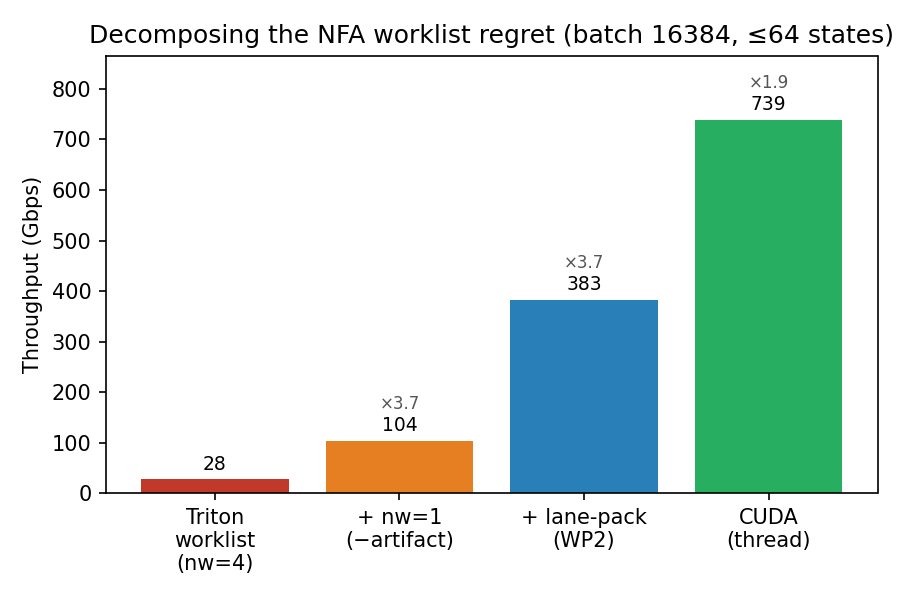
\includegraphics[width=\columnwidth]{figures/fig_decomposition.png}
\caption{The NFA worklist regret decomposes into artifact, recoverable, and irreducible.}
\label{fig:decomp}\end{figure}
\begin{figure}[t]\centering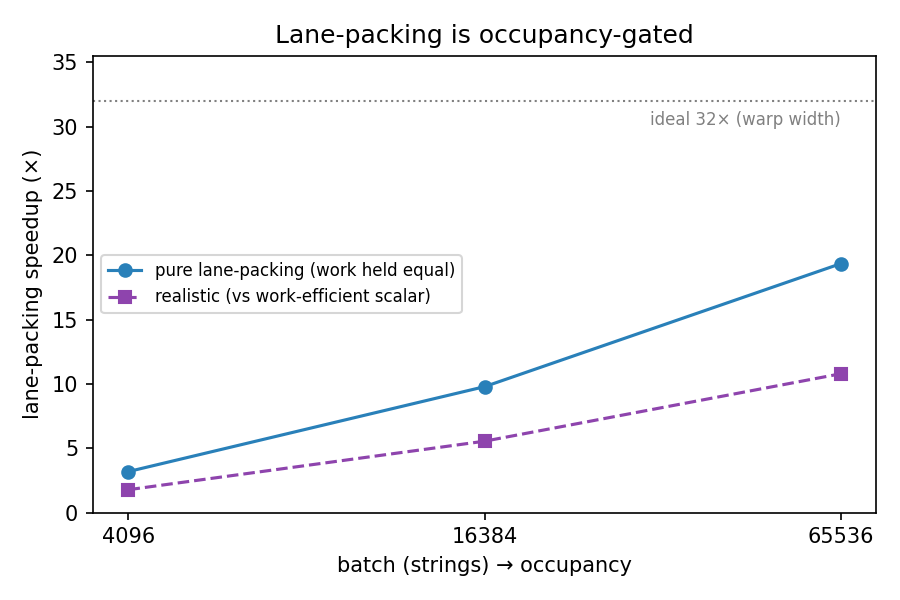
\includegraphics[width=\columnwidth]{figures/fig_occupancy_gating.png}
\caption{Lane-packing is occupancy-gated.}\label{fig:occ}\end{figure}
\begin{figure}[t]\centering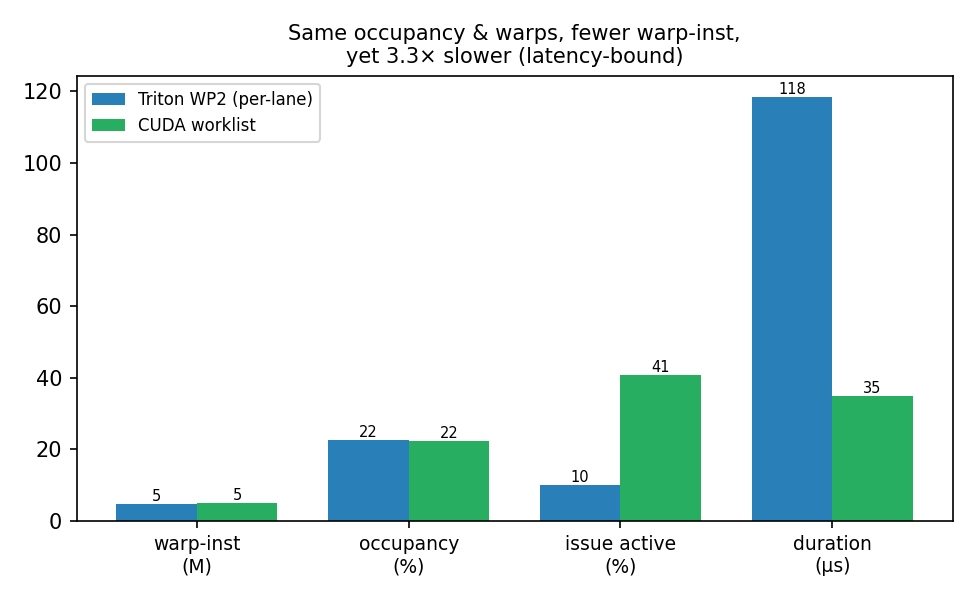
\includegraphics[width=\columnwidth]{figures/fig_mechanism.png}
\caption{Same occupancy and warps, fewer warp-instructions---yet slower (latency-bound).}
\label{fig:mech}\end{figure}
\begin{figure}[t]\centering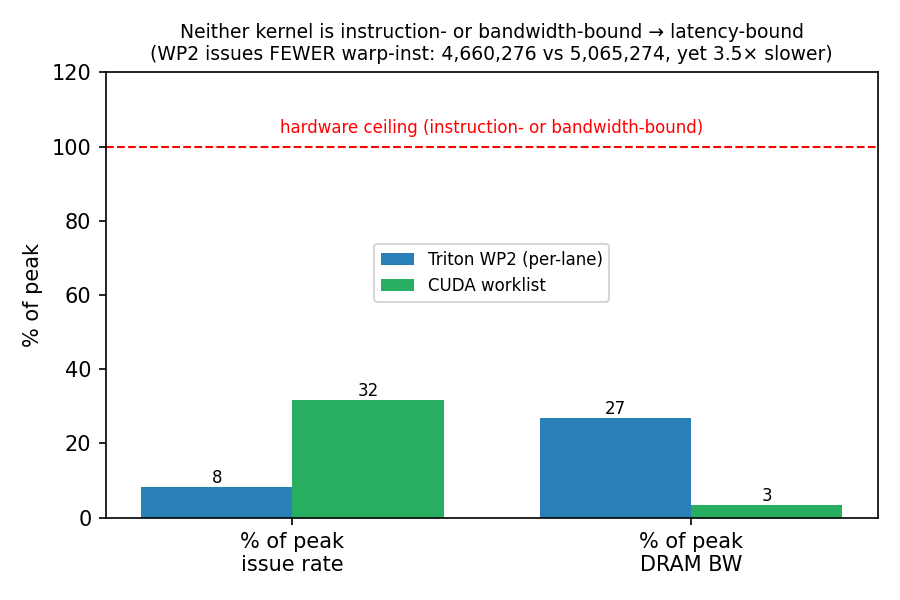
\includegraphics[width=\columnwidth]{figures/fig_roofline.png}
\caption{Neither kernel is instruction- or bandwidth-bound.}\label{fig:roof}\end{figure}
\begin{figure}[t]\centering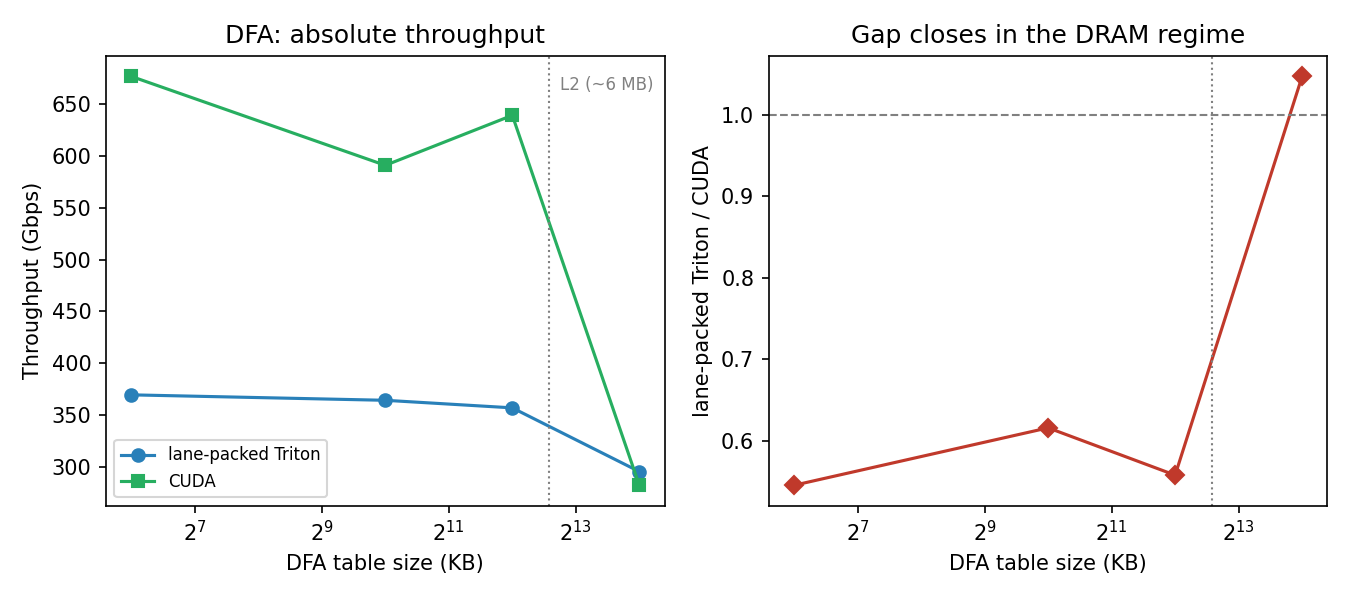
\includegraphics[width=\columnwidth]{figures/fig_dfa_crossover.png}
\caption{DFA: the gap closes in the DRAM regime.}\label{fig:dfa}\end{figure}

\bibliographystyle{unsrt}
\bibliography{refs}
\end{document}
